
\chapter{Resultat}

\begin{binge}

\section{Läromaterialet}

Läromaterialet blev i slutändan en sammanvävning av domänspecifika språk som modellerar fysik, och lärotext som förklarar kopplingen mellan fysiken och de domänspecifika språken. Figur \ref{fig:smakprov_laromaterial} visar ett kort utdrag ur läromaterialet. Där ser man hur domänspecifika språk och lärotext är sammanvävda.

\begin{figure}[tph]
  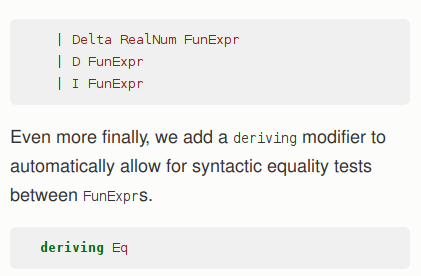
\includegraphics[width=\linewidth]{figure/smakprov_laromaterial.png}
  \caption{Ett smakprov över hur det resulterande läromaterialet ser ut. Lärotext är framför den ljusgrå bakgrunden medan Haskell-kod för domänspecifika språk är framför den mörkgrå.}
  \label{fig:smakprov_laromaterial}
\end{figure}

I läromaterialet finns även bilder. Figur \ref{fig:smakprov_bild_laromaterial} är ett exempel på en bild ur läromaterialet. Speciellt att notera är den medvetet oseriösa ritningstekniken som är tänkt att vara rolig och muntra upp läsaren.

\begin{figure}
  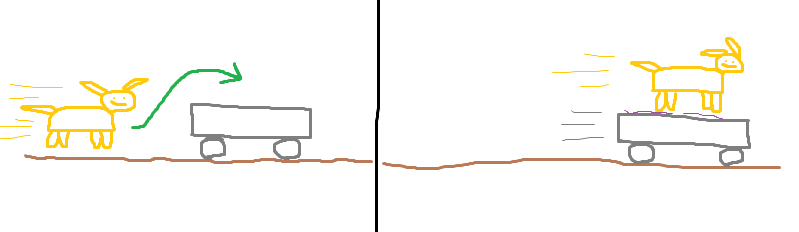
\includegraphics[width=\linewidth]{figure/smakprov_bild_laromaterial.png}
  \caption{Exempel på en bild ur läromaterialet. Bilden visar hur en hund springer och hoppar upp på en stillastående vagn. När hunden landat rör sig hunden och vagnen med en ny, gemensam hastighet.}
  \label{fig:smakprov_bild_laromaterial}
\end{figure}

Läromataterialet behandlar ett flertal områden inom fysik och matematik som används inom fysik. Fokuset är på klassisk mekanik samt till det området tillhörande matematik. I sin fullständighet är de behandlade områdena

\begin{itemize}
  \item Bevis
  \item Dimensioner
  \item Matematisk analys
  \item Vektorer
  \item Tillämpningar av ovanstående
\end{itemize}

I \textit{bevis}-kapitlet presenteras bevisföringen med hjälp av Haskells typsystem. Det exemplifieras genom att kinematiska formler bevisas.

\textit{Dimensioner} behandlar dimensioner, storheter och enheter inom fysiken. Dimensioner införs på typnivå i Haskell för att kunna visa på likheten mellan Haskells typsystem och hur man måste förhålla sig till dimensioner inom fysiken.

I \textit{matematisk analys} konstrueras ett syntaxträd för algebraiska uttryck och funktioner. Därefter implementeras symbolisk derivering och integrering på syntaxträdet.

\textit{Vektorer} implementerar vektorer och vektoroperationer i Haskell. Lagar som ska gälla för vektorer implementeras och testas.

I läromataterialet finns, förutom de fyra ovanstående grundläggande områdena, även tillämpningar av dem på exempelproblem. Till exempel används dimensioner till att lösa problem med fritt fall. De tillämpningar som behandlats är

\begin{itemize}
  \item Gundbräda
  \item Krafter på lådor
\end{itemize}

Läromaterialet blev publicerat på en hemsida\cite{LYAP} och all källkod finns tillgänglig på projektets GitHub-repository.\cite{LYAP_repo} Texten är skriven på engelska.

\section{Återkoppling från testgrupp}

För att utvärdera huruvida läromaterialet är intressant och hjälpsamt har vi
haft en informell återkoppling med en testgrupp. TODO: Skriv mer när vi
faktiskt gjort detta.

\end{binge}
